%% https://www.redblobgames.com/grids/hexagons/
%% https://www.redblobgames.com/grids/hexagons/implementation.html
%% https://github.com/jclopes/hive
%% https://github.com/josephroquedev/hive-engine

\documentclass[ngerman, gray]{sdqassignment}

\lecture{Programmieren}
\semester{Sommersemester 2019}
\lecturer{Prof.\,Dr.\,Ralf H. Reussner}
\group{Software Design and Quality (SDQ)}
\ilias{https://sdqweb.ipd.kit.edu/wiki/Programmieren}
\mail{programmieren-vorlesung@ipd.kit.edu}
\assignment{Abschlussaufgabe 2}
\points{20 Punkte}
\releasedate{29.07.2019, ca.\,13:00 Uhr}
\praktomatdate{12.08.2019, 13:00 Uhr}
\duedate{27.08.2019, 06:00 Uhr}
\version{Version 1.0}

\begin{document}

\hinweise{3}[\java{java.lang}, \java{java util}, \java{java.util.regex} und \java{java.util.function}]

\clause{Abgabemodalitäten}

Die Praktomat"=Abgabe wird am \textbf{Montag, den 12.08.2019 um 13:00 Uhr}, freigeschaltet. Achten Sie unbedingt darauf, Ihre Dateien im Praktomaten bei der richtigen Aufgabe vor Ablauf der Abgabefrist hochzuladen.
\begin{itemize}
    \item Geben Sie Ihre Klassen zu Aufgabe A als \txt{*.java}"=Dateien ab.
\end{itemize}

%\clearpage
\setcounter{figure}{0}
\task{Jagd nach Mister~X}{20}
In dieser Abschlussaufgabe soll ein Legespiel mit sechseckigen Spielsteinen für zwei Spieler implementiert werden.
Die Spieler mit ihren Spielsteinen werden jeweils durch die Farben \enquote{Infrarot} und \enquote{Ultraviolett} unterschieden. Ziel des Spiels ist es, den \enquote{Mister~X} des Gegners komplett einzuschließen und gleichzeitig zu verhindern, dass der Gegner den eigenen Mister~X einschließt. Die Spielsteine, welche Mister~X einschließen, können teilweise eigene, teilweise gegnerische Spielsteine sein. Wer zuerst den Mister~X des Gegners eingeschlossen hat, gewinnt.

\begin{figure}[ht]
    \centering
    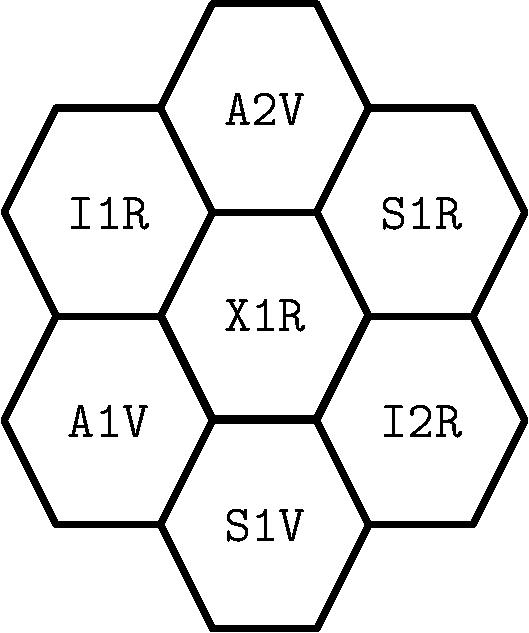
\includegraphics[scale=0.45]{Niederlage}
    \label{fig:niederlage}
    \caption{Der infrarote Mister~X ist eingeschlossen.}
\end{figure}

\subsection{Spielsteine}
\label{steine}
Jeder Spieler hat elf sechseckige Spielsteine. Jede Art von Spielstein wird über einen Buchstaben klassifiziert. Zusätzlich erhält jede Art von Spielstein noch zur eindeutigen Identifikation eine Zahl.
\begin{itemize}
    \item einen Mister~X: \txt{X1}
    \item zwei Agenten: \txt{A1} und \txt{A2}
    \item zwei Spione: \txt{S1} und \txt{S2}
    \item drei Ermittler: \txt{E1}, \txt{E2} und \txt{E3}
    \item drei Informanten: \txt{I1}, \txt{I2} und \txt{I3}
\end{itemize}

Zur Zuordnung der Spielsteine zu den zwei Spieler, werden noch zusätzlich entweder \txt{R} (Infrarot) oder \txt{V} (Ultraviolett) als Kürzel für die Farbe an die Kennung eines Spielsteins mit angehängt. Zum Beispiel wäre \txt{X1R} der \enquote{infrarote Mister~X} und \txt{A2V} wäre der \enquote{zweite ultraviolette Agent}.

\subsubsection{Berührungskanten}
\label{kanten}
Um darzustellen, wie Spielsteine nebeneinander platziert werden, werden die Berührungskanten angegeben. Hierbei wird zwischen dem Zielstein und dem Zugstein unterschieden. Der Zielstein ist der bereits im Spiel befindliche Spielstein, welcher im aktuellen Zug nicht bewegt wird. Der Zugstein ist der Stein, welcher im aktuellen Zug neu ins Spiel eingebracht oder bewegt wird. Eine Berührungskante beziehen sich auf die Kanten des Zielsteins, welcher der Zugstein im Laufe oder am Ende eines Zuges berührt.

\begin{description}
    \item[0] Zugstein wird auf den Zielstein (Oben) gelegt.
    \item[1] Zugstein wird an die oberste Kante (Norden) des Zielsteins gelegt.
    \item[2] Zugstein wird an die linke oberste Kante (Nordost) des Zielsteins gelegt.
    \item[3] Zugstein wird an die linke untere Kante (Südost) des Zielsteins gelegt.
    \item[4] Zugstein wird an die unterste Kante (Süden) des Zielsteins gelegt.
    \item[5] Zugstein wird an die rechte untere Kante (Südwest) des Zielsteins gelegt.
    \item[6] Zugstein wird an die rechte oberste Kante (Nordwest) des Zielsteins gelegt.
\end{description}

\begin{figure}[ht]
    \centering
    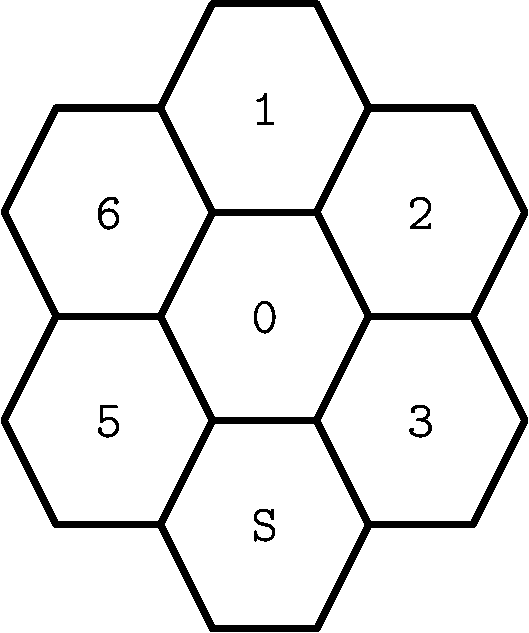
\includegraphics[scale=0.45]{Kanten}
    \label{fig:kanten}
    \caption{Die sieben \hyperref[kanten]{Berührungskanten} eines Spielsteins.}
\end{figure}

\subsubsection{Textuelle Beschreibung}
\label{textuell}
Ein Spielstein wird zusammen mit den ihn berührenden Steinen textuell beschrieben. Diese textuelle Beschreibung beginnt mit der Kennung (siehe \cref{steine}) des zu repräsentierenden Spielsteins, gefolgt von den Berührungskanten mit dem jeweils an ihnen anliegenden Spielstein. Dabei werden die Kennungen der Spielsteine und die Zahlen der Berührungskanten jeweils durch ein Leerzeichen voneinander getrennt und die Berührungskanten werden nach den ihnen zugeordneten Zahlen aufsteigend geordnet. Wenn an einer Berührungskante kein Spielstein anliegt, wird diese bei der Beschreibung übersprungen und nicht mit ausgegeben. So ist die textuelle Beschreibung des Spielsteines \txt{X1R} in \cref{fig:niederlage} wie folgt: \txt{X1R 1 A2V 2 S1R 3 I2R 4 S1V 5 A1V 6 I1R}

\subsection{Spielablauf}
\label{ablauf}
Ein Spieler beginnt, indem er einen Spielstein aus seinem Vorrat auf das Spielfeld legt. Der andere Spieler legt einen seiner Spielsteine so daneben, dass die beiden Spielsteine sich an einer Kante berühren. Anschließend sind beide Spieler abwechselnd an der Reihe, einen Spielstein entweder einzusetzen oder zu bewegen.

\subsubsection{Einsetzen der Spielsteine}
Ein neuer Spielstein kann bei jedem Zug eingesetzt werden. Außer im ersten Spielzug darf ein Spielstein niemals angrenzend an einen gegnerischen Spielstein eingesetzt werden. Man muss nicht alle Spielsteine einsetzen, um das Spiel zu gewinnen. Ein einmal eingesetzter Spielstein kann jedoch nicht wieder entfernt werden. Auch müssen alle neuen Spielsteine auf das Spielfeld gelegt werden. Ein neuer Spielstein kann auch in ein umgebenes Loch eingesetzt werden, da die Regel zur Bewegungsfreiheit nicht für das Ablegen neuer Spielsteine gilt.

\subsubsection{Der Schauplatz}
Die im Spiel befindlichen Spielsteine bilden das Spielfeld, auch \enquote{Schauplatz} genannt.

\subsubsection{Einsetzen von Mister~X}
Mister~X kann in einem der ersten vier Züge eingesetzt werden. Spätestens im vierten Zug muss er eingesetzt worden sein.

\subsubsection{Bewegung der Spielsteine}
Bis zum Einsetzen des Mister~X dürfen andere Spielsteine zwar eingesetzt, aber nicht bewegt werden. Erst wenn der eigene Mister~X im Spiel ist, kann ein Spieler bei jedem Zug entscheiden, ob er einen neuen Spielstein einsetzt oder einen bereits vorhandenen bewegt. Jeder Geheimdienstler hat dabei eigene Regeln, nach denen er sich im Schauplatz bewegen kann. Ein Spielstein darf am Ende seiner Bewegung auch an einen oder mehrere gegnerische Spielsteine angrenzen. Ein Spielstein muss immer an mindestens einen anderen angrenzen. Ist ein Spielstein die einzige Verbindung zwischen zwei Teilen des Schauplatzes, darf er nicht bewegt werden.

\subsection{Arten von Geheimdienstlern}
Jede Art von Geheimdienstler (Spielstein) hat ihre eigenen Regeln, nach denen er ziehen darf.

\subsubsection{Mister~X}
\label{misterx}
Mister~X kann pro Zug nur ein Feld weit ziehen. Trotz dieser Einschränkung kann er mit einer Bewegung zum richtigen Zeitpunkt die Pläne des Gegners vereiteln.

\begin{figure}[ht]
    \centering
    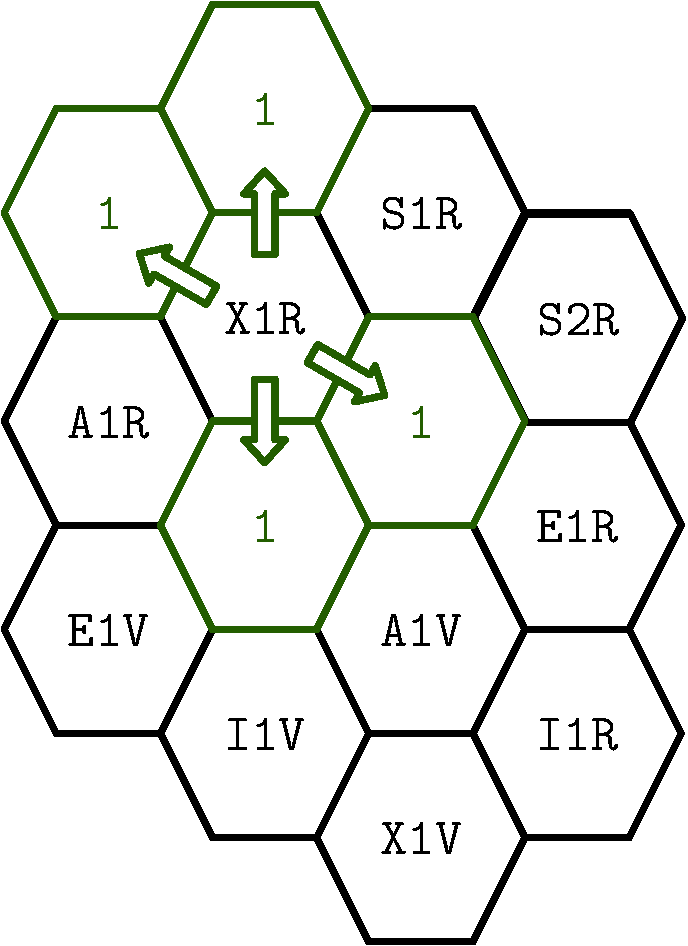
\includegraphics[scale=0.45]{MisterX}
    \label{fig:misterx}
    \caption{Von dieser Position aus kann der infrarote \hyperref[misterx]{Mister~X} auf eine der vier angegeben Position ziehen.}
\end{figure}

\subsubsection{Agent}
\label{agent}
Der Agent bewegt sich genau wie Mister~X nur ein Feld weit. Im Gegensatz zu anderen Geheimdienstlern kann er jedoch auch auf den Schauplatz gezogen werden und andere Spielsteine überdecken. Ein Spielstein, der unter einem Agent liegt, kann nicht bewegt werden. Beim Einsetzen eines neuen Spielsteins ist die Farbe des oben sitzenden Agenten für den gesamten Stapel ausschlaggebend. Der Agent kann sich auf dem Schauplatz von einem Spielstein zum nächsten bewegen, und hierbei auch direkt mehrere Ebenen auf- oder absteigen. Ein Agent kann aber auch wieder hinabsteigen und dabei auch umschlossene Felder betreten, die für die meisten Geheimdienstler nicht erreichbar sind. Der einzige Weg, einen Agent auf dem Schauplatz zu blockieren, ist, einen anderen Agent darauf zu setzen. Alle Agenten können übereinandergestapelt werden. Beim Einsetzen wird der Agent wie alle anderen Geheimdienstler behandelt. Er kann nicht direkt auf einem anderen Spielstein eingesetzt werden, sondern sich erst in einem der folgenden Züge dorthin bewegen.

\begin{figure}[ht]
    \centering
    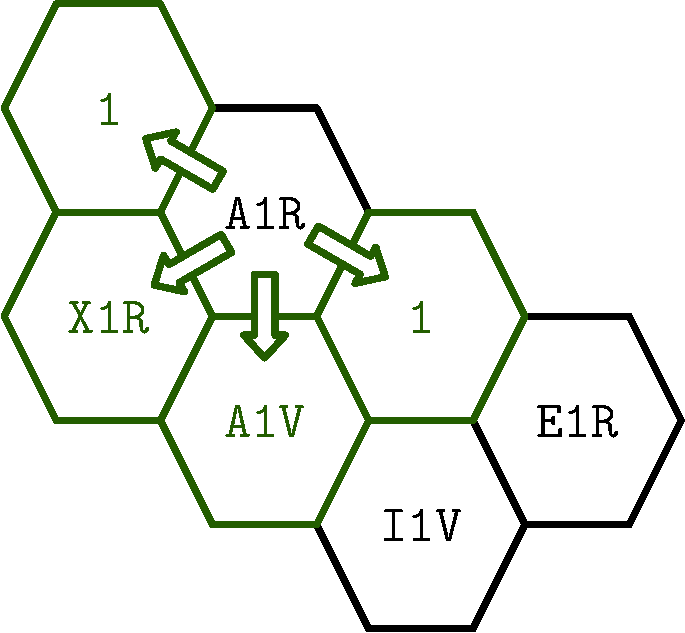
\includegraphics[scale=0.45]{Agent}
    \label{fig:agent}
    \caption{Von seiner jetzigen Position aus kann der infrarote \hyperref[agent]{Agent} auf eine der vier angegeben Positionen gezogen werden.}
\end{figure}

\subsubsection{Spion}
\label{spion}
Der Spion bewegt sich nicht wie die anderen Geheimdienstler außen am Schauplatz entlang. Stattdessen springt er von seiner Position aus in gerader Linie über eine beliebige Anzahl aneinandergrenzender Spielsteine -- jedoch mindestens einen -- auf den dahinterliegenden freien Platz. Auf diese Weise kann der Spion auch auf komplett eingeschlossene Felder gelangen. Spion können auch über einen Stapel von mehreren Spielsteinen springen. Beispielsweise, kann er in \cref{fig:spion} nicht in die Lücke oder über die Lücke hinweg auf die mit \txt{X} gekennzeichneten Position springen.

\begin{figure}[ht]
    \centering
    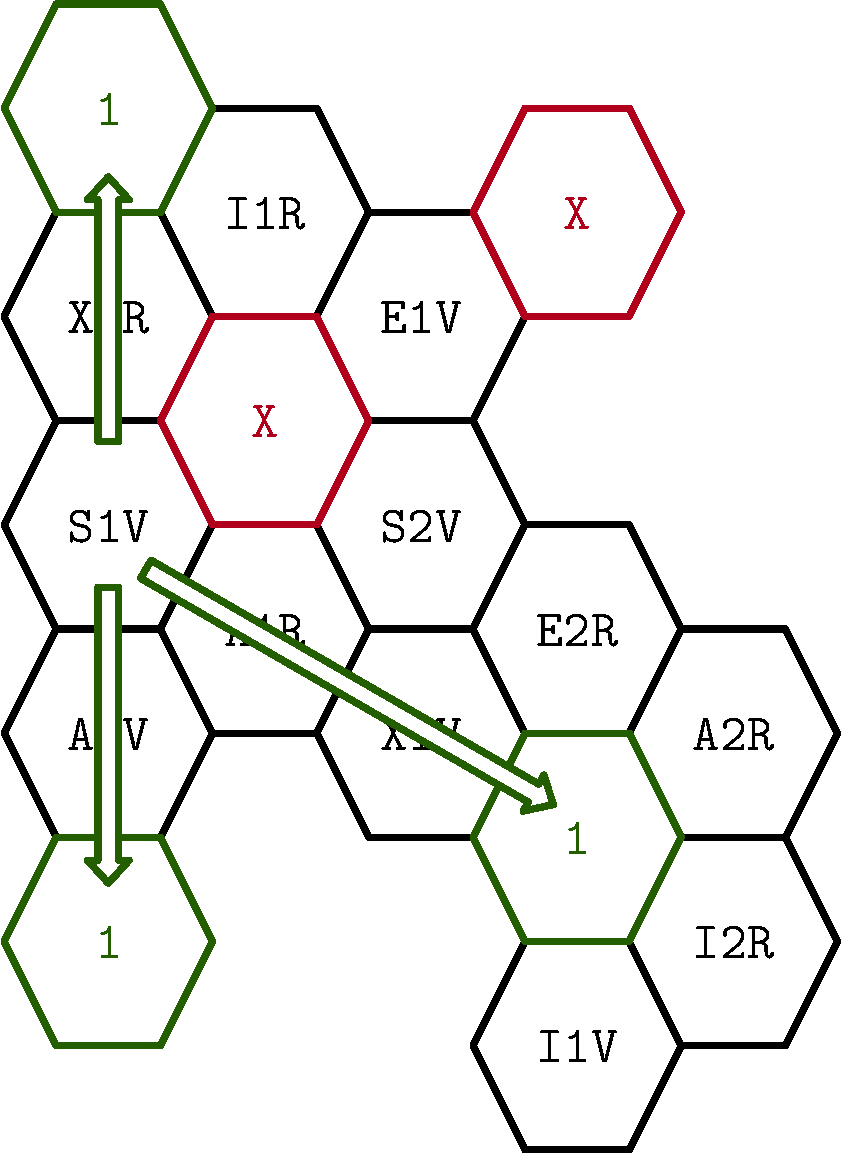
\includegraphics[scale=0.45]{Spion}
    \label{fig:spion}
    \caption{Von seiner jetzigen Position aus kann der violette \hyperref[spion]{Spion}  auf eine der drei angegeben Positionen springen.}
\end{figure}


\subsubsection{Ermittler}
\label{ermittler}
Der Ermittler bewegt sich bei jedem Zug genau drei Felder weit. Dabei darf er kein Feld zweimal betreten und auch nicht zu seiner Ausgangsposition zurückkehren. Auch kann ein Ermittler sich nicht in einen Raum bewegen, in den er nicht passt. Bei jedem seiner drei Schritte muss er Kontakt mit mindestens einem Geheimdienstler halten, den er vor diesem Schritt bereits berührt. Er darf also nicht von sämtlichen Spielsteinen, die er in einer Position berührt, getrennt und an einen anderen Spielstein angelegt werden.

\begin{figure}[ht]
    \centering
    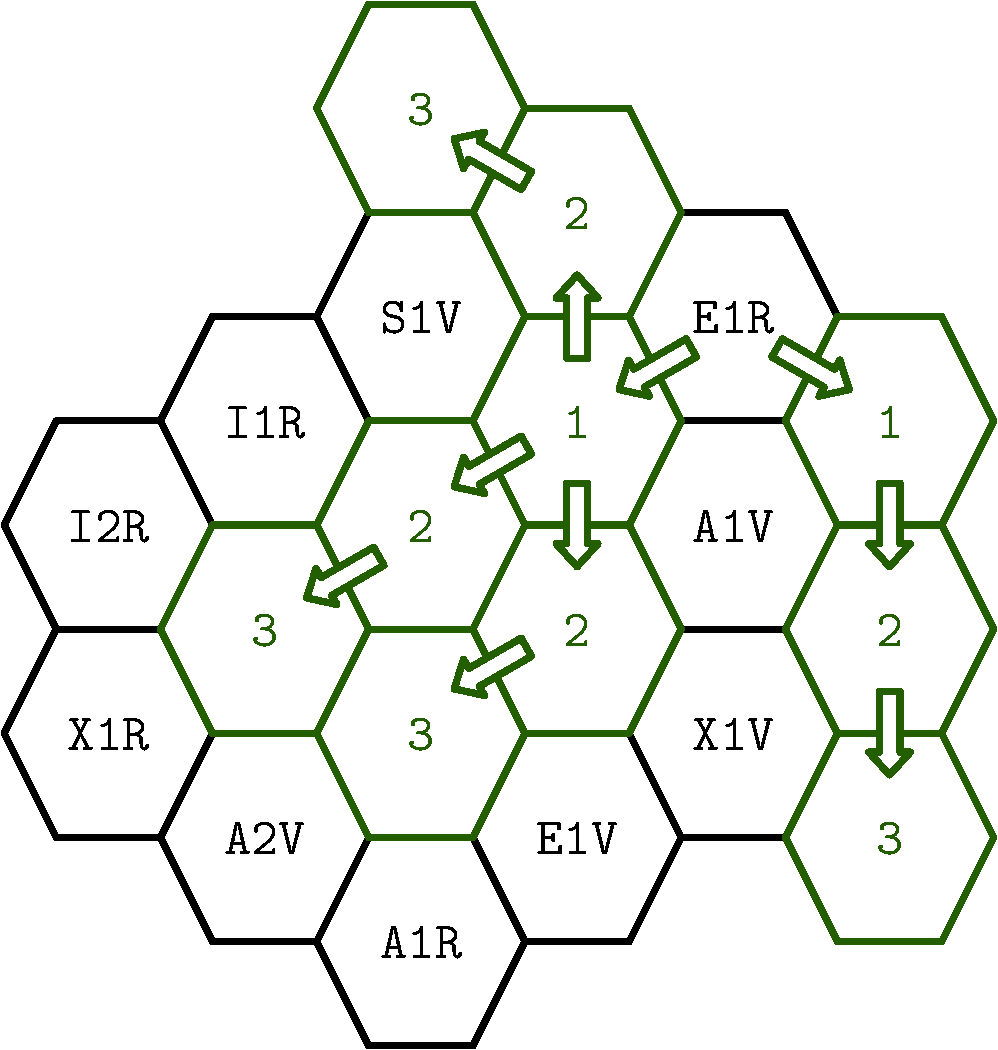
\includegraphics[scale=0.45]{Ermittler}
    \label{fig:ermittler}
    \caption{Von seiner jetzigen Position aus kann der infrarote \hyperref[ermittler]{Ermittler} Ermittler auf eine der vier angegebenen Positionen ziehen. Er kann nicht in einem Schritt auf die mit 2 markierte Position links von ihm ziehen, da er dort kein Geheimdienstler berühren würde, welcher vor diesem Schritt bereits berührt hat.}
\end{figure}

\subsubsection{Informant}
\label{informant}
Der Informant kann sich von seiner Position aus auf jedes andere Feld um den Schauplatz herumbewegen, sofern die allgemeinen Bewegungsregeln eingehalten werden. Diese Bewegungsfreiheit macht den Informanten zu einer der wertvollsten Spielfiguren.

\begin{figure}[ht]
    \centering
    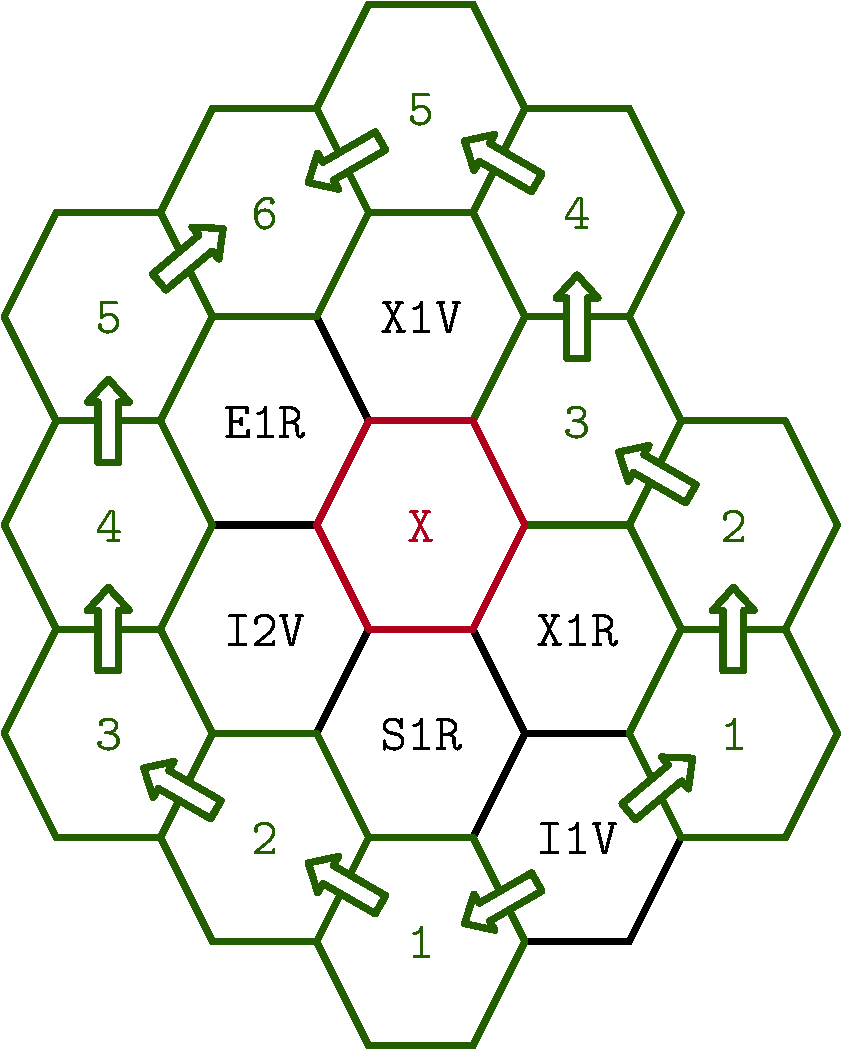
\includegraphics[scale=0.45]{Informant}
    \label{fig:informant}
    \caption{In diesem Fall kann der \hyperref[informant]{Informant} Informant auf ein der elf angegeben Positionen ziehen, jedoch nicht auf das freie Feld im Zentrum des Schauplatzes (siehe \cref{freiheit}).}
\end{figure}

\subsection{Einschränkungen}
\subsubsection{Der Schauplatz}
Die Spielsteine auf dem Spielfeld müssen jederzeit miteinander verbunden sein. Kein Spielstein darf alleine (ohne Verbindung zum Schauplatz) sein. Der Schauplatz darf auch nicht geteilt werden.

\begin{figure}[ht]
    \centering
    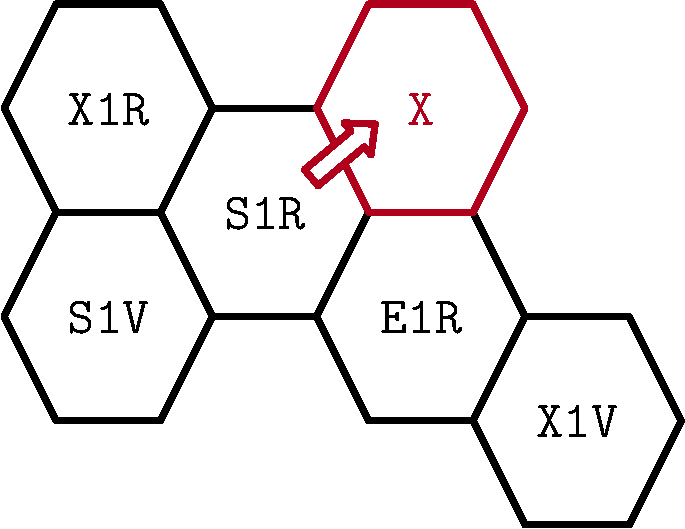
\includegraphics[scale=0.45]{Schauplatz1}
    \label{fig:schauplatz1}
    \caption{Der Zug der infraroten Spions würde den Schauplatz in zwei Teile spalten.}
\end{figure}

\begin{figure}[ht]
    \centering
    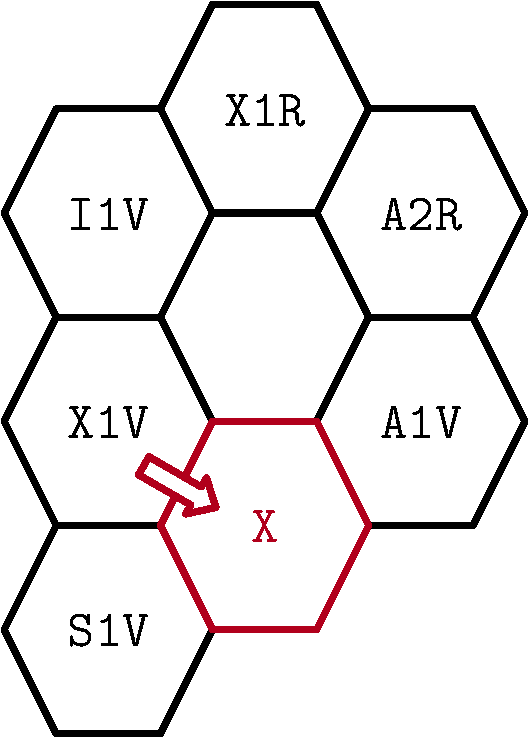
\includegraphics[scale=0.45]{Schauplatz2}
    \label{fig:schauplatz2}
    \caption{Auch dieser Zug ist nicht erlaubt: Der violette Mister~X darf nicht in die angegebene Position gezogen werden, obwohl er den Schauplatz dort wieder verbinden würde, denn während seiner Bewegung wäre der Schauplatz vorübergehend geteilt.}
\end{figure}

\subsubsection{Bewegungsfreiheit}
\label{freiheit}
Die Spielsteine können nur durch Schieben bewegt werden. Ist ein Spielstein so weit eingeschlossen, dass er nicht mehr aus seiner Position herausgeschoben werden kann, kann er nicht bewegt werden. Ebenso kann kein Spielstein auf ein Feld gezogen werden, das so weit umschlossen ist, dass der Spielstein nicht hineingeschoben werden kann. Die einzigen Ausnahmen sind der Spion, welcher in eine Lücke hinein- und aus einer Lücke herausspringen kann, sowie der Agent, der hinein- und herausklettern kann. Beim Einsetzen darf ein Spielstein auf ein umschlossenes Feld gesetzt werden, wenn die anderen Regeln zum Einsetzen dies zulassen, der neue Spielstein also keinen gegnerischen Spielstein berührt.

\begin{figure}[ht]
    \centering
    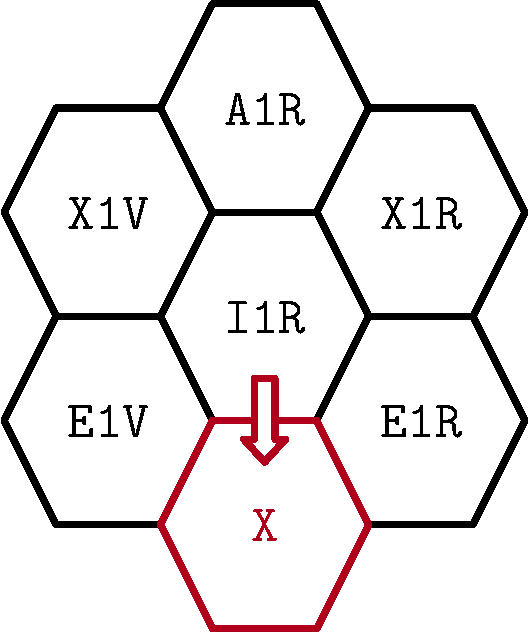
\includegraphics[scale=0.45]{Bewegungsfreiheit1}
    \hfil
    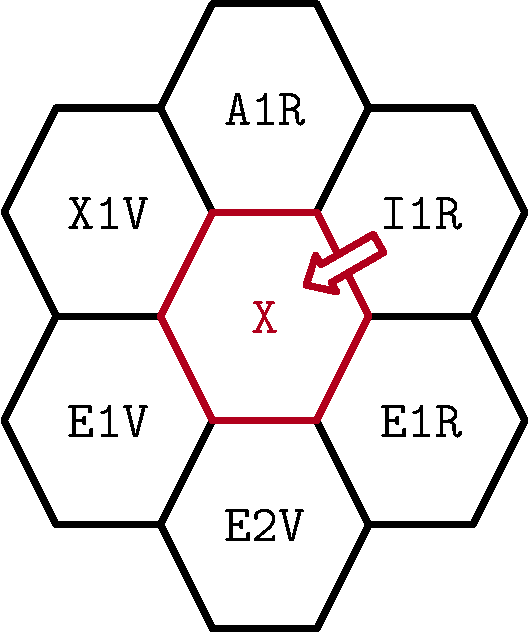
\includegraphics[scale=0.45]{Bewegungsfreiheit3}
    \hfil
    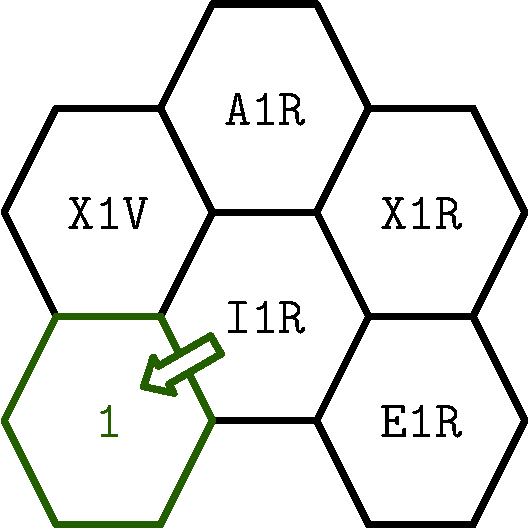
\includegraphics[scale=0.45]{Bewegungsfreiheit2}
    \label{fig:freiheit}
    \caption{Drei unabhängig Beispiele für zwei ungültige und einen gültigen Zug.}
\end{figure}

\subsubsection{Bewegungsunfähigkeit}
\label{passen}
Wenn ein Spieler weder einen neuen Spielstein einsetzen, noch einen Spielstein im Schauplatz bewegen kann, muss dieser passen, das heißt der Gegner ist sofort wieder am Zug. Auch wenn ein Spieler nicht bewegungsunfähig ist, kann er passen. Jedoch darf ein Spieler nicht passen, bevor er seinen Mister~X eingesetzt hat. Wenn ein Spieler passt, zählt dies für diesen als ein Zug. Das Spiel wird auf diese Weise fortgesetzt, bis der Spieler wieder einen Spielstein einsetzen oder bewegen kann oder sein Mister~X eingeschlossen ist. Wenn beide Spieler allerdings direkt hintereinander passen endet das Spiel unentschieden.

\subsubsection{Spielende}
\label{ende}
Das Spiel endet, sobald ein Mister~X komplett von anderen Spielsteinen eingeschlossen ist. Die Farbe der 6 Spielsteine, die den Mister~X umgeben, ist irrelevant. Der Spieler, dessen Mister~X eingeschlossen wird, verliert das Spiel, es sei denn, derselbe Zug schließt beide Mister~X ein. In diesem Fall endet das Spiel unentschieden.

\subsection{Interaktive Benutzerschnittstelle}
Nach dem Start nimmt Ihr Programm über die Konsole mittels \java{Terminal.readLine()} Eingaben, welche im Folgenden näher spezifiziert werden. Nach Abarbeitung einer Eingabe wartet Ihr Programm auf weitere Eingaben, bis das Programm irgendwann durch die Eingabe der Zeichenfolge \txt{quit} beendet wird.

\subsubsection{Fehlermeldungen}
Achten Sie darauf, dass durch Ausführung der folgenden Befehle die zuvor definierten Spielregeln nicht verletzt werden und geben Sie in diesen Fällen immer eine aussagekräftige Fehlermeldung aus. Auch wenn die Benutzereingabe nicht dem vorgegebenen Format entspricht, ist eine Fehlermeldung auszugeben. Nach der Ausgabe einer Fehlermeldung soll das Programm wie erwartet fortfahren und wieder auf die nächste Eingabe warten. Jede Fehlermeldung muss mit \txt{Error,} beginnen und darf keine Zeilenumbrüche enthalten. Den weiteren Text der Fehlermeldung dürfen Sie frei wählen, er sollte jedoch sinnvoll sein.

\subsubsection{Automatische Tests}
Da wir automatische Tests Ihrer interaktiven Benutzerschnittstelle durchführen, müssen die Ausgaben exakt den Vorgaben entsprechen. Insbesondere sollen sowohl Klein- und Großbuchstaben als auch die Leerzeichen und Zeilenumbrüche genau übereinstimmen. Geben Sie auch keine zusätzlichen Informationen aus. Beginnen Sie frühzeitig mit dem Einreichen, um Ihre Lösung dahingehend zu testen, und verwenden Sie das Forum, um eventuelle Unklarheiten zu klären.

\subsubsection{Platzhalter}
Beachten Sie, dass bei der Beschreibung der Eingabe- und Ausgabeformate die Wörter zwischen spitzen Klammen (\txt{<} und \txt{>}) für Platzhalter stehen, welche bei der konkreten Ein- und Ausgabe durch Werte ersetzt werden. Diese eigentlichen Werte enthalten bei der Ein- und Ausgabe keine spitzen Klammern. Vergleichen Sie hierzu auch die jeweiligen Beispielabläufe.

\paragraph{\txt{<Zugstein>} und \txt{<Zielstein>}} Ein Spielstein wird, wie in \cref{steine} beschrieben, eindeutig durch seine Art, seinen Zahl und seine Farbe bestimmt.

\paragraph{\txt{<Kante>}} Eine Berührungskante wird, wie in \cref{kanten} beschrieben, eindeutig als eine einstellige ganze Zahl bestimmt.

\paragraph{\txt{<Pfad>}} Ein Pfad ist eine Folge aus \txt{<Kante>} und \txt{<Zielstein>} Paaren. Eine Kante bezieht sich immer auf den ihr nachfolgenden Zielstein. Die Kante und der Zielstein eines Paares, sowie die Paare untereinander, werden durch jeweils ein Leerzeichen voneinander getrennt.
% Pfad muss immer an einem angrenzenden Stein entlang. Er kann nicht in einem Schritt auf die mit 2 markierte Position links von ihm ziehen, da er dort kein Geheimdienstler berühren würde, welcher vor diesem Schritt bereits berührt hat.

\paragraph{\txt{<PLAYER>}} Die Farbe eines Spielers; entweder \txt{INFRARED} oder \txt{ULTRAVIOLET}.

\subsection{Befehle}
Nach jedem regelkonformen Zug (\txt{start}-, \txt{place}-, \txt{move}- und \txt{pass}"=Befehl) wechselt der aktive Spieler. Die Befehle \txt{place}, \txt{move}, \txt{pass} und \txt{print} dürfen nur während einem aktiven Spiel eingegeben werden. Leerzeichen werden durch \visiblespace dargestellt.

\subsubsection{Ausgabeformat}
Wenn in den Befehlen nichts weiter spezifiziert wird, gelten die folgenden Spezifikationen für das Ausgabeformat für alle Befehle. Bei dem Auftreten eines Fehlers wird eine Fehlermeldung ausgebenden. Wenn der eingegebene Befehl gemäß den Spezifikationen erfolgreich ausgeführt wurde, wird in einer Zeile nur \txt{OK} ausgegeben. Wenn das Spiel regulär endet, wird in einer Zeile nur \txt{WINNER <PLAYER>}[showspaces=true] ausgegeben, wobei \txt{<PLAYER>} die Farbe des Spielers ist, welcher gewonnen hat. Wenn das Spiel in einem Unentschieden endet, wird in einer Zeile nur \txt{DRAW} ausgegeben.

\subsubsection{Der \txt{start}"=Befehl}
Der Befehl startet ein neues aktives Spiel. Wird der Befehl während eines laufenden Spiels eingebeben, wird dieses abgebrochen und ein neues Spiel gestartet. Den Spielregeln entsprechend wird der angegebene Zugsteins als erster Spielstein gelegt. Die Farbe des Zugsteins bestimmt implizit den beginnenden Spieler.
\paragraph{Eingabeformat}\txt{start <Zugstein>}[showspaces=true]

\subsubsection{Der \txt{place}"=Befehl}
Der Befehl legt den Regeln entsprechend den Zugstein an die Kante des Zielsteins.
\paragraph{Eingabeformat}\txt{place <Zugstein> <Kante> <Zielstein>}[showspaces=true]

\subsubsection{Der \txt{move}"=Befehl}
Der Befehl bewegt den Regeln entsprechend den Zugstein an die Kante des Zielstein. Das letzte Paar des Pfades bestimmt die Kante des Zielsteins, an welche der Zugstein am Ende seiner Bewegung liegt. Bei der Bewegung eines Spion besteht der Pfad aus lediglich aus einem Paar, welches den freien Platz bestimmen, auf welchen der Spion springt (siehe \cref{spion}).
\paragraph{Eingabeformat}\txt{move <Zugstein> <Pfad>}[showspaces=true]

\subsubsection{Der \txt{pass}"=Befehl}
Der Befehl wechselt den aktiven Spieler (siehe \cref{passen}).
\paragraph{Eingabeformat}\txt{pass}

\subsubsection{Der \txt{print}"=Befehl}
Der Befehl gibt den aktuellen Zustand des Schauplatzes in der folgenden spezifizierten textuellen Beschreibung aus.
\paragraph{Eingabeformat}\txt{print}
\paragraph{Ausgabeformat} Ein Spielstein wird zeilenweise wie in \cref{textuell} beschrieben ausgegeben. Dabei werden die aktuell im Spiel befindlichen Steine wie folgt zeilenweise geordnet: 1.~\txt{X1R}, 2.~\txt{A1R}, 3.~\txt{A2R}, 4.~\txt{S1R}, 5.~\txt{S2R}, 6.~\txt{E1R}, 7.~\txt{E2R}, 8.~\txt{E3R}, 9.~\txt{I1R}, 10.~\txt{I2R}, 11.~\txt{I3R}, 12.~\txt{X1V}, 13.~\txt{A1V}, 14.~\txt{A2V}, 15.~\txt{S1V}, 16.~\txt{S2V}, 17.~\txt{E1V}, 18.~\txt{E2V}, 19.~\txt{E3V}, 20.~\txt{I1V}, 21.~\txt{I2V}, 22.~\txt{I3V}. Wenn sich ein Spielstein nicht im Schauplatz befindet, wird dieser bei der textuellen Beschreibung übersprungen und nicht mit ausgegeben.

\subsubsection{Der \txt{quit}"=Befehl}
Der parameterlose Befehl ermöglicht es, die Jagd nach Mister~X vollständig zu beenden. Beachten Sie, dass hierfür keine Methoden wie \java{System.exit()} oder \java{Runtime.exit()} verwendet werden dürfen.
\paragraph{Eingabeformat}\txt{quit}

\subsection{Beispielablauf}
Beachten Sie auch, dass bei den folgenden Beispielabläufen die Eingabezeilen mit dem \txt{>}"=Zeichen gefolgt von einem Leerzeichen eingeleitet werden. Diese beiden Zeichen sind ausdrücklich kein Bestandteil des eingegebenen Befehls, sondern dienen nur der Unterscheidung zwischen Ein- und Ausgabezeilen.

\end{document}
